\documentclass{article}
\usepackage{caption, float, graphicx}
\usepackage[dvipsnames]{xcolor}
\captionsetup[table]{skip=1em}

\title{ESE 326: Final Project}
\author{Eric Stewart \& Gabriel Minton}
\date{November 2024}

\begin{document}

\maketitle

\section{Exploratory Analysis}

\color{Aquamarine}
% Do subplots for petal/ sepal lengths/ widths
Caption: Plots color-coded for each of the 3 species.

\begin{figure}[H]
	\centering
	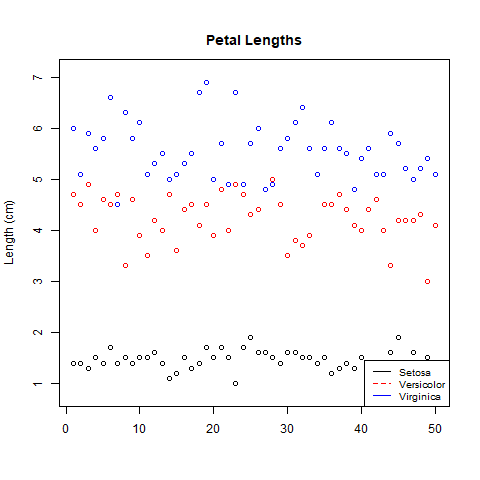
\includegraphics[width=.5\textwidth]{petal_length.png}
	\caption{Petal lengths of each species}
\end{figure}

\section{Inference Analysis}


\end{document}
